% ============================================================
%  KickSneakApp — Prezentare susținere licență (Beamer, light)
%  Olaru David · Universitatea „Ovidius" din Constanța · 2026
%  Compilare: pdflatex main.tex (x2)
%  Stil: minimal — doar tehnologii, iconițe și capturi;
%        prezentatorul vorbește peste slide-uri.
% ============================================================
\documentclass[aspectratio=169,11pt]{beamer}

\usepackage[T1]{fontenc}
\usepackage[utf8]{inputenc}
\usepackage[romanian]{babel}
\usepackage{lmodern}
\usepackage{graphicx}
\usepackage{tikz}
\usetikzlibrary{shapes.geometric, arrows.meta, positioning, fit, calc}

% ---------- Identitate vizuală KickSneak (light + olive/lime) ----------
\definecolor{ksbg}{HTML}{FFFFFF}
\definecolor{kstext}{HTML}{171A0B}
\definecolor{ksolive}{HTML}{566E0B}
\definecolor{kslime}{HTML}{A3C51B}
\definecolor{ksmuted}{HTML}{6A6F5E}
\definecolor{kschip}{HTML}{EFF3D8}
\definecolor{kschiptext}{HTML}{3D4A12}
\definecolor{kssoft}{HTML}{F4F5EF}

\setbeamercolor{background canvas}{bg=ksbg}
\setbeamercolor{normal text}{fg=kstext}
\setbeamercolor{frametitle}{fg=ksolive,bg=ksbg}
\setbeamercolor{title}{fg=ksolive}
\setbeamercolor{structure}{fg=ksolive}
\setbeamercolor{footline}{fg=ksmuted}
\setbeamerfont{frametitle}{series=\bfseries,size=\Large}
\setbeamertemplate{navigation symbols}{}
\setbeamertemplate{footline}{%
  \hfill\scriptsize\color{ksmuted}KickSneakApp — Olaru David\quad|\quad\insertframenumber/\inserttotalframenumber\hspace{2em}\vspace{1ex}}
% linie lime sub titlul de frame
\addtobeamertemplate{frametitle}{}{\vspace{-2mm}{\color{kslime}\hrule height 1.2pt}\vspace{1mm}}

% Chip cu cuvânt-cheie
\newcommand{\chip}[1]{\setlength{\fboxsep}{4pt}\colorbox{kschip}{\textcolor{kschiptext}{\strut\footnotesize\textbf{#1}}}\hspace{1.2mm}}
% Badge tehnologie (text)
\newcommand{\techbadge}[1]{\setlength{\fboxsep}{5pt}\colorbox{kstext}{\textcolor{kslime}{\strut\textbf{#1}}}}
% Iconiță cu fallback text
\newcommand{\techicon}[2]{\IfFileExists{icons/#1.png}{\includegraphics[height=8mm]{icons/#1.png}}{\techbadge{#2}}}
% Screenshot cu ramă subtilă
\newcommand{\shot}[2]{\IfFileExists{screenshots/#1}{\setlength{\fboxsep}{0pt}\setlength{\fboxrule}{0.6pt}{\color{ksmuted}\fbox{\includegraphics[width=#2]{screenshots/#1}}}}{}}

% Stiluri TikZ pentru diagrame
\tikzset{
  tbl/.style={rectangle, rounded corners=2pt, draw=ksolive, fill=kschip,
              text=kstext, font=\tiny\bfseries, inner sep=3pt, minimum height=5.5mm},
  tblaux/.style={rectangle, rounded corners=2pt, draw=ksmuted!70, fill=kssoft,
              text=ksmuted, font=\tiny, inner sep=3pt, minimum height=5mm},
  fk/.style={-{Latex[length=1.6mm]}, draw=ksmuted, thin},
  fkmain/.style={-{Latex[length=1.8mm]}, draw=ksolive, semithick},
  lbl/.style={font=\tiny, text=ksmuted, midway, fill=ksbg, inner sep=1pt},
}

\title{KickSneakApp}
\author{Olaru David}
\date{2026}

\begin{document}

% ============================================================
% 1. TITLU
% ============================================================
\begin{frame}[plain]
  \begin{center}
    \IfFileExists{sigla.png}{
\includegraphics[height=17mm]{sigla.png}\\[2mm]}{}
    {\color{ksmuted}\small UNIVERSITATEA „OVIDIUS" DIN CONSTANȚA\\
    FACULTATEA DE MATEMATICĂ ȘI INFORMATICĂ\\
    Specializarea Informatică}\\[7mm]
    {\color{ksmuted}\normalsize LUCRARE DE LICENȚĂ}\\[3mm]
    {\color{ksolive}\Huge\bfseries KickSneakApp}\\[6mm]
    {\color{kslime}\rule{60mm}{1.2pt}}\\[6mm]
    \begin{columns}
      \column{0.5\textwidth}\centering
        {\color{ksmuted}\footnotesize Coordonator științific}\\
        {\color{kstext}\small\textbf{Lect. Dr. Andrei Rusu}}
      \column{0.5\textwidth}\centering
        {\color{ksmuted}\footnotesize Absolvent}\\
        {\color{kstext}\small\textbf{Olaru David}}
    \end{columns}
    \vspace{6mm}
    {\color{ksmuted}\footnotesize Constanța — 2026}
  \end{center}
\end{frame}

% ============================================================
% 2. CUPRINS
% ============================================================
\begin{frame}{Cuprins}
  \vspace{2mm}
  \begin{columns}[t]
    \column{0.5\textwidth}
    \begin{enumerate}\setlength{\itemsep}{6pt}\color{kstext}
      \item Aplicația principală
      \item Aplicația de administrare
      \item Baza de date
      \item Notificări live \& Web Push
      \item Instrumente \& infrastructură
    \end{enumerate}
    \column{0.5\textwidth}
    \begin{enumerate}\setcounter{enumi}{5}\setlength{\itemsep}{6pt}\color{kstext}
      \item Securitate
      \item AI — sistemul de recomandare
      \item LLM open-source — chat cu Ollama
      \item Mulțumiri
    \end{enumerate}
  \end{columns}
\end{frame}

% ============================================================
% 3. APLICAȚIA PRINCIPALĂ
% ============================================================
\begin{frame}{Aplicația principală}
  \begin{center}
    \techicon{react}{React}\hspace{5mm}\techicon{vite}{Vite}\hspace{5mm}\techicon{typescript}{TypeScript}\hspace{5mm}\techicon{dotnet}{.NET 10}\hspace{5mm}\techicon{postgresql}{PostgreSQL}\hspace{5mm}\techicon{redis}{Redis}\\[1.5mm]
    \techbadge{REST API}\hspace{2mm}\techbadge{WebSocket / SignalR}\hspace{2mm}\techbadge{Stripe}\hspace{2mm}\techbadge{Elasticsearch}
  \end{center}
  \begin{columns}[T]
    \column{0.42\textwidth}
    \centering
    \shot{home-ai.png}{0.52\linewidth}
    \column{0.56\textwidth}
    \centering
    \shot{product-history.png}{0.86\linewidth}
  \end{columns}
  \vspace{2mm}
  \begin{center}
    \chip{Catalog 10.000+}\chip{Căutare \& filtre}\chip{Favorite \& coș}\chip{Checkout Stripe}\chip{Licitații live}\chip{Recenzii}\chip{Retururi}\chip{Profil seller}
  \end{center}
\end{frame}

% ============================================================
% 4. APLICAȚIA ADMIN
% ============================================================
\begin{frame}{Aplicația de administrare}
  \begin{center}
    \techbadge{Next.js}\hspace{2mm}\techbadge{Server Actions}\hspace{2mm}\techbadge{Prisma}\hspace{2mm}\techicon{postgresql}{PostgreSQL}\hspace{5mm}\techbadge{WebSocket}\hspace{2mm}\techicon{docker}{Docker}
  \end{center}
  \vspace{1mm}
  \begin{columns}[T]
    \column{0.62\textwidth}
    \centering
    \shot{admin-orders.png}{0.9\linewidth}
    \column{0.36\textwidth}
    \centering
    \shot{admin-broadcast-crop.png}{0.56\linewidth}
  \end{columns}
  \vspace{2mm}
  \begin{center}
    \chip{Dashboard KPI}\chip{Comenzi}\chip{Retururi}\chip{Recenzii}\chip{Verificare stoc — kanban}\chip{Broadcast push}\chip{Chat suport live}\chip{Utilizatori \& vânzători}
  \end{center}
\end{frame}

% ============================================================
% 5. BAZA DE DATE (1/2) — Catalog & Comerț
% ============================================================
\begin{frame}{Baza de date (1/2) — catalog \& comerț}
  \centering
  \vspace{2mm}
  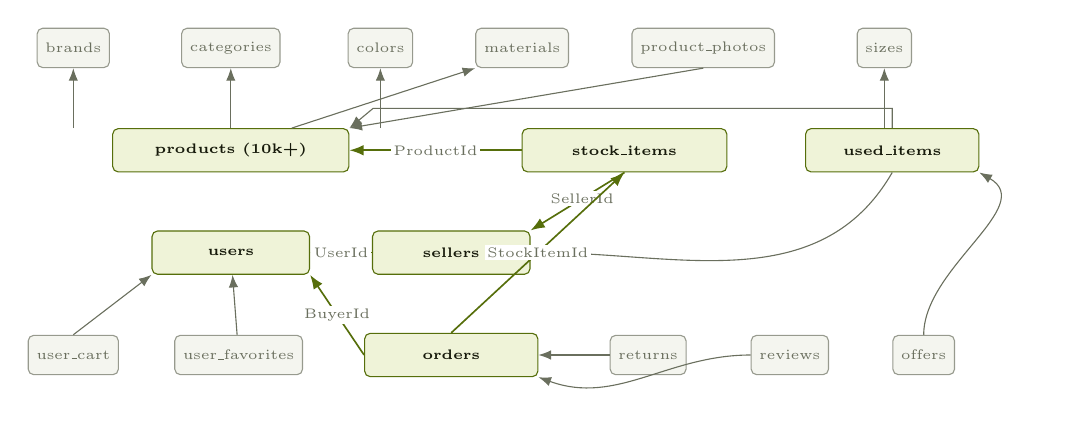
\begin{tikzpicture}[x=1cm,y=1cm]
    \node[tblaux] (brands)     at (0.6,3.3)  {brands};
    \node[tblaux] (categories) at (2.6,3.3)  {categories};
    \node[tblaux] (colors)     at (4.5,3.3)  {colors};
    \node[tblaux] (materials)  at (6.3,3.3)  {materials};
    \node[tblaux] (photos)     at (8.6,3.3)  {product\_photos};
    \node[tblaux] (sizes)      at (10.9,3.3) {sizes};
    \node[tbl, minimum width=30mm] (products) at (2.6,2.0)  {products (10k+)};
    \node[tbl, minimum width=26mm] (stock)    at (7.6,2.0)  {stock\_items};
    \node[tbl, minimum width=22mm] (used)     at (11.0,2.0) {used\_items};
    \node[tbl, minimum width=20mm] (users)    at (2.6,0.7)  {users};
    \node[tbl, minimum width=20mm] (sellers)  at (5.4,0.7)  {sellers};
    \node[tblaux] (cart)    at (0.6,-0.6)  {user\_cart};
    \node[tblaux] (favs)    at (2.7,-0.6)  {user\_favorites};
    \node[tbl, minimum width=22mm] (orders) at (5.4,-0.6) {orders};
    \node[tblaux] (returns) at (7.9,-0.6)  {returns};
    \node[tblaux] (reviews) at (9.7,-0.6)  {reviews};
    \node[tblaux] (offers)  at (11.4,-0.6) {offers};
    \draw[fk] (products.north -| brands.south) -- (brands.south);
    \draw[fk] (products) -- (categories);
    \draw[fk] (products.north -| colors.south) -- (colors.south);
    \draw[fk] (products.20) -- (materials.south west);
    \draw[fk] (photos.south) -- (products.north east);
    \draw[fkmain] (stock) -- node[lbl]{ProductId} (products);
    \draw[fk] (stock.north -| sizes.south) -- (sizes.south);
    \draw[fkmain] (stock.south) -- node[lbl, pos=0.45]{SellerId} (sellers.north east);
    \draw[fk] (used.north) |- ($(products.north east)+(0.3,0.25)$) -- (products.north east);
    \draw[fk] (used.south) to[out=-120,in=0] (sellers.east);
    \draw[fkmain] (sellers) -- node[lbl]{UserId} (users);
    \draw[fkmain] (orders.north) -- node[lbl, pos=0.5]{StockItemId} (stock.south);
    \draw[fkmain] (orders.west) -- node[lbl]{BuyerId} (users.south east);
    \draw[fk] (returns) -- (orders);
    \draw[fk] (reviews.west) to[out=180,in=-20] (orders.south east);
    \draw[fk] (cart.north) -- (users.south west);
    \draw[fk] (favs) -- (users);
    \draw[fk] (offers.north) to[out=90,in=-30] (used.south east);
  \end{tikzpicture}
\end{frame}

% ============================================================
% 6. BAZA DE DATE (2/2) — Licitații & interacțiune
% ============================================================
\begin{frame}{Baza de date (2/2) — licitații, interacțiune \& mesagerie}
  \centering
  \vspace{2mm}
  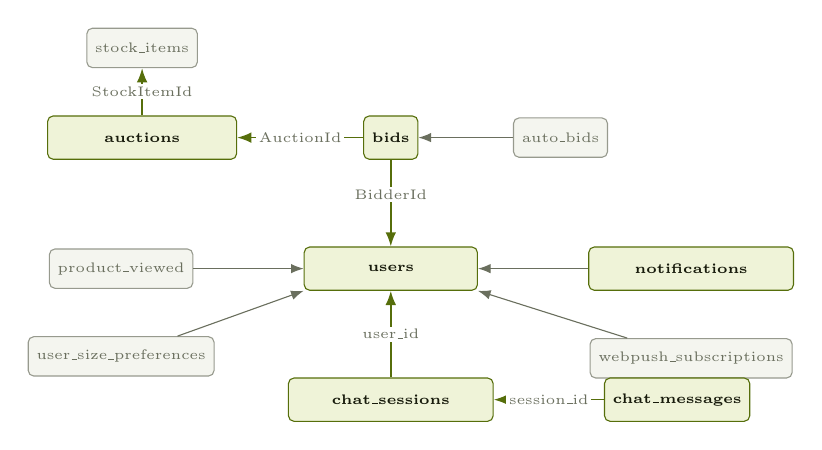
\begin{tikzpicture}[node distance=6mm and 10mm]
    \node[tbl, minimum width=24mm] (auctions) {auctions};
    \node[tbl, right=16mm of auctions] (bids) {bids};
    \node[tblaux, right=12mm of bids] (autobids) {auto\_bids};
    \node[tblaux, above=6mm of auctions] (stock2) {stock\_items};
    \node[tbl, below=11mm of bids, minimum width=22mm] (users2) {users};
    \node[tblaux, left=14mm of users2] (viewed) {product\_viewed};
    \node[tblaux, below=6mm of viewed] (sizepref) {user\_size\_preferences};
    \node[tbl, right=14mm of users2, minimum width=26mm] (notif) {notifications};
    \node[tblaux, below=6mm of notif] (webpush) {webpush\_subscriptions};
    \node[tbl, below=11mm of users2, minimum width=26mm] (sessions) {chat\_sessions};
    \node[tbl, right=14mm of sessions] (messages) {chat\_messages};
    \draw[fkmain] (auctions) -- node[lbl]{StockItemId} (stock2);
    \draw[fkmain] (bids) -- node[lbl]{AuctionId} (auctions);
    \draw[fkmain] (bids) -- node[lbl, pos=0.4]{BidderId} (users2);
    \draw[fk] (autobids) -- (bids);
    \draw[fk] (viewed) -- (users2);
    \draw[fk] (sizepref) -- (users2.south west);
    \draw[fk] (notif) -- (users2);
    \draw[fk] (webpush) -- (users2.south east);
    \draw[fkmain] (sessions) -- node[lbl]{user\_id}(users2);
    \draw[fkmain] (messages) -- node[lbl]{session\_id} (sessions);
  \end{tikzpicture}\\[4mm]
  \chip{Row-Level Security}\chip{Semnale AI: views · favorites · orders}\chip{Chat: rol DB dedicat}
\end{frame}

% ============================================================
% 7. NOTIFICĂRI LIVE + WEB PUSH
% ============================================================
\begin{frame}{Notificări live \& Web Push}
  \begin{center}
    \techbadge{SignalR}\hspace{2mm}\techbadge{WebSocket}\hspace{2mm}\techbadge{Web Push}\hspace{2mm}\techbadge{VAPID}\hspace{2mm}\techbadge{Service Worker}
  \end{center}
  \vspace{1mm}
  \begin{columns}[T]
    \column{0.56\textwidth}
    \centering
    \shot{home-logged.png}{\linewidth}\\[1mm]
    {\tiny\color{ksmuted} Broadcast din admin $\rightarrow$ toast live la utilizator}
    \column{0.42\textwidth}
    \centering
    \shot{webpush-windows.png}{\linewidth}\\[1mm]
    {\tiny\color{ksmuted} Notificare Web Push la nivel de sistem de operare}
  \end{columns}
  \vspace{2mm}
  \begin{center}
    \chip{Bid nou}\chip{Outbid}\chip{Update comandă}\chip{Ofertă nouă}\chip{Broadcast admin}
  \end{center}
\end{frame}

% ============================================================
% 8. TOOLS
% ============================================================
\begin{frame}{Instrumente \& infrastructură}
  \begin{center}
    \techicon{grafana}{Grafana}\hspace{5mm}\techbadge{Prometheus}\hspace{2mm}\techbadge{Loki}\hspace{2mm}\techbadge{Elasticsearch}\hspace{2mm}\techbadge{Kibana}\hspace{2mm}\techicon{redis}{Redis}\hspace{5mm}\techicon{docker}{Docker}
  \end{center}
  \vspace{1mm}
  \begin{columns}[T]
    \column{0.5\textwidth}
    \centering
    \shot{grafana.png}{\linewidth}\\[1mm]
    {\tiny\color{ksmuted} Observabilitate: metrici .NET + log-uri centralizate}
    \column{0.5\textwidth}
    \centering
    \shot{docker-desktop.png}{\linewidth}\\[1mm]
    {\tiny\color{ksmuted} 18+ containere orchestrate cu Docker Compose}
  \end{columns}
\end{frame}

% ============================================================
% 9. SECURITATE
% ============================================================
\begin{frame}{Securitate}
  \vspace{1mm}
  \begin{center}
    {\color{ksmuted}\small Autentificare \& autorizare}\\[1.5mm]
    \chip{Firebase Auth — JWT}\chip{Middleware autentificare}\chip{RBAC — 6 roluri PostgreSQL}\chip{Row-Level Security}\\[4mm]
    {\color{ksmuted}\small Apărare în adâncime}\\[1.5mm]
    \chip{Rate limiter — Redis}\chip{Trace-ID per cerere}\chip{Logging structurat}\chip{EF Core ORM — anti SQL injection}\\[2mm]
    \chip{Validare server-side}\chip{CORS restrictiv}\chip{Secrete în variabile de mediu}\chip{Plăți delegate — Stripe}\\[5mm]
    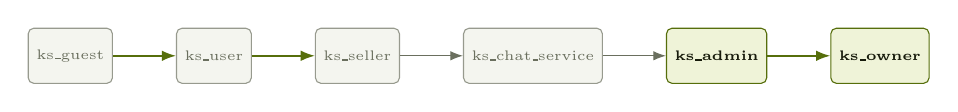
\begin{tikzpicture}[node distance=8mm, every node/.style={font=\scriptsize}]
      \node[tblaux, minimum height=7mm] (guest) {ks\_guest};
      \node[tblaux, right=of guest, minimum height=7mm] (user) {ks\_user};
      \node[tblaux, right=of user, minimum height=7mm] (seller) {ks\_seller};
      \node[tblaux, right=of seller, minimum height=7mm] (chat) {ks\_chat\_service};
      \node[tbl, right=of chat, minimum height=7mm] (admin) {ks\_admin};
      \node[tbl, right=of admin, minimum height=7mm] (owner) {ks\_owner};
      \draw[fkmain] (guest) -- (user);
      \draw[fkmain] (user) -- (seller);
      \draw[fk] (seller) -- (chat);
      \draw[fk] (chat) -- (admin);
      \draw[fkmain] (admin) -- (owner);
    \end{tikzpicture}
  \end{center}
\end{frame}

% ============================================================
% 10. AI — SISTEMUL DE RECOMANDARE
% ============================================================
\begin{frame}{AI — sistemul de recomandare}
  \begin{center}
    \techbadge{PyTorch}\hspace{2mm}\techbadge{Rețea neuronală}\hspace{2mm}\techbadge{Recommender}\hspace{2mm}\techbadge{Reranker}\hspace{2mm}\techbadge{Flask}\hspace{2mm}\techbadge{Quartz}
  \end{center}
  \vspace{2mm}
  \begin{columns}[T]
    \column{0.46\textwidth}
    \centering
    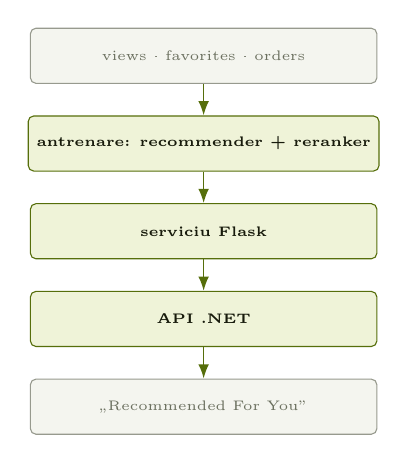
\begin{tikzpicture}[node distance=4mm, every node/.style={font=\scriptsize}]
      \node[tblaux, minimum width=44mm, minimum height=7mm] (sig) {views · favorites · orders};
      \node[tbl, below=of sig, minimum width=44mm, minimum height=7mm] (train) {antrenare: recommender + reranker};
      \node[tbl, below=of train, minimum width=44mm, minimum height=7mm] (flask) {serviciu Flask};
      \node[tbl, below=of flask, minimum width=44mm, minimum height=7mm] (api) {API .NET};
      \node[tblaux, below=of api, minimum width=44mm, minimum height=7mm] (ui) {„Recommended For You"};
      \draw[fkmain] (sig) -- (train);
      \draw[fkmain] (train) -- (flask);
      \draw[fkmain] (flask) -- (api);
      \draw[fkmain] (api) -- (ui);
    \end{tikzpicture}
    \column{0.52\textwidth}
    \centering
    \shot{home-ai.png}{0.86\linewidth}
  \end{columns}
  \vspace{1.5mm}
  \begin{center}
    \chip{Personalizare per utilizator}\chip{Fallback cold-start}\chip{Reantrenare periodică}\chip{Căutare cu AI}
  \end{center}
\end{frame}

% ============================================================
% 11. LLM OPEN-SOURCE — CHAT CU OLLAMA
% ============================================================
\begin{frame}{LLM open-source — chat suport cu Ollama}
  \begin{center}
    \techbadge{Llama 3.1 — 8B}\hspace{2mm}\techbadge{Ollama}\hspace{2mm}\techicon{go}{Go}\hspace{5mm}\techbadge{WebSocket}\hspace{2mm}\techicon{postgresql}{PostgreSQL}
  \end{center}
  \vspace{1mm}
  \begin{columns}[T]
    \column{0.5\textwidth}
    \centering
    \shot{chat-user.png}{0.95\linewidth}\\[1mm]
    {\tiny\color{ksmuted} AI-ul răspunde cu datele reale ale comenzii}
    \column{0.5\textwidth}
    \centering
    \shot{chat-admin-taken.png}{0.95\linewidth}\\[1mm]
    {\tiny\color{ksmuted} Operatorul preia conversația de la AI}
  \end{columns}
  \vspace{2mm}
  \begin{center}
    \chip{100\% local}\chip{Streaming token-cu-token}\chip{Proxy Go — I/O garantat}\chip{Analiză de intenție}\chip{Escaladare la operator}
  \end{center}
\end{frame}

% ============================================================
% 12. MULȚUMIRI
% ============================================================
\begin{frame}[plain]
  \begin{center}
    \vspace{14mm}
    {\color{ksolive}\Huge\bfseries Vă mulțumesc pentru atenție!}\\[8mm]
    {\color{kslime}\rule{60mm}{1.2pt}}\\[6mm]
    {\color{kstext}\large KickSneakApp}\\[3mm]
    {\color{ksmuted}\small React · .NET 10 · PostgreSQL · Redis · Elasticsearch · Docker\\
     SignalR · Web Push · Stripe · PyTorch · Ollama (Llama 3.1)}\\[10mm]
    {\color{ksmuted}\footnotesize Olaru David — Universitatea „Ovidius" din Constanța\\
    Coordonator: Lect. Dr. Andrei Rusu · 2026}
  \end{center}
\end{frame}

\end{document}
